\chapter{An'alisis de Fourier}
\pagenumbering{arabic}
\setcounter{page}{1}


\section{Resumen: Series de Fourier}

\subsection{Propiedades Generales} Si $f(\theta)$ es una funci'on (real o compleja) peri'odica, de periodo $2\pi$, su \textbf{serie de Fourier} es dada por
\begin{equation}\label{sf1}
 f(\theta) =\frac{a_0}{2}  +\sum_{n=1}^\infty 
\big(a_n\cos(n\theta) + b_n\sen(n\theta)\big).
\end{equation}
Recuerde que las funciones $\left\lbrace\cos(n\theta),\sen(n\theta)\right\rbrace_{n=0}^{\infty}$ forman una base completa para el espacio de las funciones peri'odicas de periodo $2\pi$ \cite{Arfken}.

%Si la serie de Fourier \textit{converge uniformemente} a $f$ entonces, 
Usando las relaciones de ortogonalidad 
\begin{equation}
\int_{-\pi}^\pi\cos(m\theta)\cos(n\theta)\,d\theta=\int_{-\pi}^\pi\sen(m\theta)\sen(n\theta)\,d\theta=\pi\delta_{mn},\label{eq:ortogo-sin-cos}
\end{equation}
\begin{equation}
\int_{-\pi}^\pi\cos(m\theta)\sen(n\theta)\,d\theta=0,
\end{equation}
podemos encontrar las expresiones para los \textbf{coeficientes de Fourier} $a_n$ y $b_n$\footnote{Es conveniente definir $b_0:=0$, tal como se incluye en (\ref{cf2}).}:
\begin{equation}\label{cf1}
a_n =\frac{1}{\pi}\int_{-\pi}^\pi f(\theta)\cos(n\theta)\,d\theta, \qquad n= 0, 1, 2,\cdots .
\end{equation}
\begin{equation}\label{cf2}
b_n =\frac{1}{\pi}\int_{-\pi}^\pi f(\theta)\sen(n\theta)\,d\theta  \qquad n= 0, 1, 2,\cdots .
\end{equation}
Equivalentemente, $f(\theta)$ puede expandirse en t'erminos proporcionales a las funciones $e^{i n\theta}$, con $n=0,\pm 1,\pm 2, \cdots$:
\begin{equation}\label{sf2}
f(\theta)=\sum_{n=-\infty}^\infty c_n e^{i n\theta},
\end{equation}
donde los coeficientes (complejos) $c_n$ est'an dados por
\begin{equation}
c_n =\frac{1}{2\pi}\int_{-\pi}^\pi f(\theta) e^{-in\theta}\,d\theta .
\end{equation}
Lo anterior puede ser verificado a partir de (\ref{sf1}), (\ref{cf1}) y (\ref{cf2}) usando la relaci'on $e^{in\theta}=\cos(n\theta)+i\sen(n\theta)$, o directamente a partir de la relaci'on de ortogonalidad
\begin{equation}
\int_{-\pi}^\pi e^{i n\theta} e^{-i m \theta}\,d\theta =2\pi\delta_{nm}.
\end{equation}
Los coeficientes de las series (\ref{sf1}) y (\ref{sf2}) est'an relacionados por
\begin{equation}c_n = 
\begin{cases}
\frac{1}{2}(a_n - i b_n)\quad &\text{para } n\geq 0,\\
%\frac{a_0}{2}\quad &\text{para } n = 0\\
\frac{1}{2}(a_{-n} + i b_{-n})\quad &\text{para } n\leq -1,
\end{cases}
\end{equation} 
o bien,
\begin{equation}
a_n=c_n+c_{-n}, \qquad b_n=i(c_n-c_{-n}), \qquad n=0,1,2,\cdots .
\end{equation}

Si $f(\theta)$ es una funci'on real entonces sus respectivos coeficientes complejos $c_n$ satisfacen la relaci'on
\begin{equation}
c_n^\ast=\frac{1}{2\pi}\int_{-\pi}^\pi f(\theta)(e^{-in\theta})^\ast\,d\theta
=\frac{1}{2\pi}\int_{-\pi}^\pi f(\theta) e^{in\theta}\,d\theta=c_{-n} 
\end{equation}
donde $z^\ast$ representa el complejo conjugado de $z$.

\subsubsection{Ejemplo: Funci'on Signo}
Sea la funci'on signo (peri'odica) $f(\theta)$, definida por 
\begin{align}
f(\theta):=\left\{
\begin{array}{rl}
-1,& \theta \in [-\pi,0)\\
1,& \theta \in [0,\pi]\\
\end{array}\right. .
\end{align}
Es directo ver que por tratarse de una funci'on impar, $a_{n}=0$ para $n=0,1,2,\ldots$. Sin embargo,
\begin{align}
b_{n}&=\frac{1}{\pi}\int_{-\pi}^{0}f(\theta) \sen(n\theta)d\theta+\frac{1}{\pi}\int_{0}^{\pi}f(\theta) \sen(n\theta)d\theta\\
&=\frac{1}{\pi}\int_{-\pi}^{0}(-1) \sen(n\theta)d\theta+\frac{1}{\pi}\int_{0}^{\pi} (1) \sen(n\theta)d\theta\\
&=\frac{1}{\pi}\int_{0}^{\pi} \sen(n\theta)d\theta+\frac{1}{\pi}\int_{0}^{\pi} \sen(n\theta)d\theta\\
&=\frac{2}{\pi}\int_{0}^{\pi}\sen(n\theta)d\theta\\
&=\left.\frac{2}{\pi}\left(\frac{-\cos(n\theta)}{n}\right)\right|_{0}^{\pi}\\
&=-\frac{2}{\pi}\left(\frac{\cos(n\pi)-1}{n}\right),
\end{align}
pero como $\cos(n\pi)=(-1)^{n}$, entonces
\begin{align}
b_{n}=-\frac{2}{\pi}\left(\frac{(-1)^{n}-1}{n}\right).
\end{align}
As'i, notando que
\begin{align}
b_{n}=\left\{
\begin{array}{cl}
0, &n\text{ par}\\
\frac{4}{n \pi}, &n\text{ impar}
\end{array}
\right.,
\end{align}
podemos escribir
\begin{align}
f(\theta)=\sum_{n\text{ impar}}\frac{4}{n\pi}\sen(n\theta)=\sum_{k=0}^{\infty}\frac{4}{\pi}\frac{\sen[(2k+1)\theta]}{(2k+1)}=\sum_{k=1}^{\infty}\frac{4}{\pi}\frac{\sen[(2k-1)\theta]}{(2k-1)}.
\end{align}
Definiendo el $k$-'esimo t'ermino de la serie como 
\begin{align}
T_{k}(\theta):=\frac{4}{\pi}\frac{\sen[(2k+1)\theta]}{(2k+1)},
\end{align}
y la \textbf{serie de Fourier truncada} hasta el t'ermino $n$-'esimo en la forma
\begin{align}
S_n(\theta):=\sum_{k=0}^n T_{k}(\theta),
\end{align}
podemos graficar algunas funciones $S_n$ que, a medida que $n$ aumenta, se acercan m'as y m'as a la funci'on original.
\begin{figure}[h]
\centering
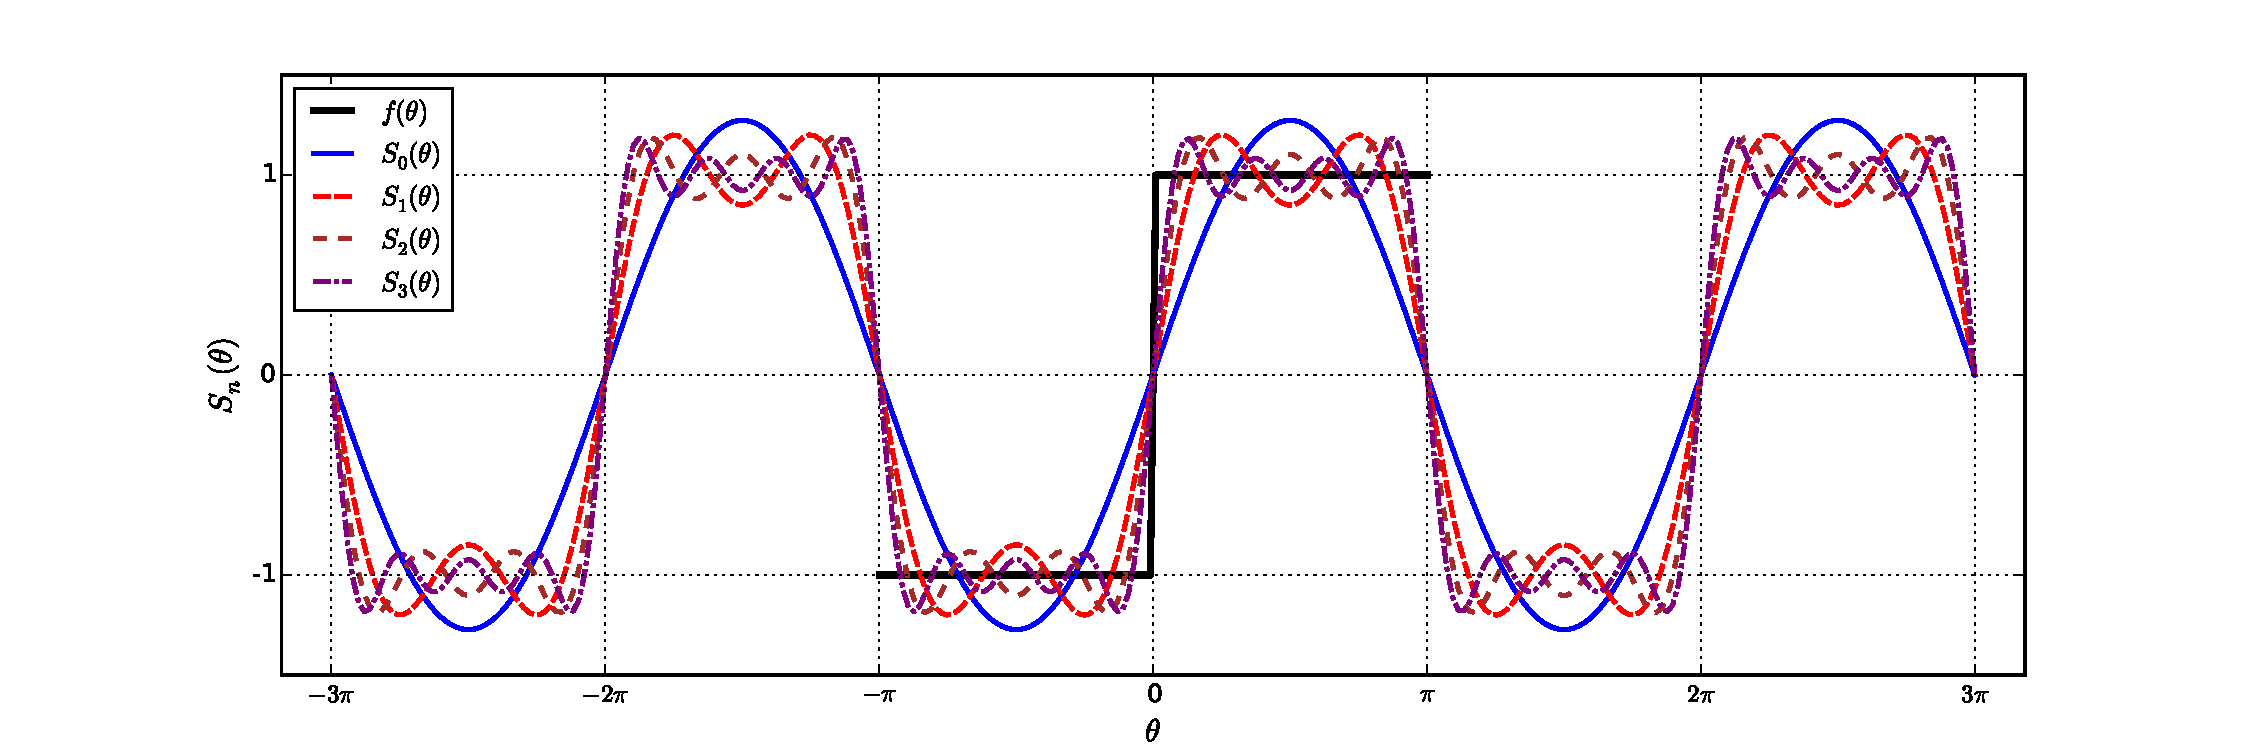
\includegraphics[scale=0.4]{figs/fig-Fourier-serie-signo.pdf}
\caption{Serie de Fourier de la funci'on Signo, truncada hasta $n=3$.}
\label{im:signo}
\end{figure}

\subsection{Convoluci'on}

La relaci'on o ``Teorema'' de Convoluci'on establece una relaci'on entre los coeficientes $C_{n}^{(1\cdot 2)}$ de la expansi'on de Fourier de la funci'on producto $f_1(\theta)f_2(\theta)$ y los respectivos coeficientes $C_{n}^{(1)}$ y $C_{n}^{(2)}$ de las funciones $f_1(\theta)$ y $f_2(\theta)$.

\begin{align}
c_n^{(1\cdot 2)} &= \frac{1}{2\pi}\int_{-\pi}^\pi f_1(\theta)f_2(\theta)e^{-in\theta}\,d\theta \\
 &= \frac{1}{2\pi}\sum_m \int_{-\pi}^\pi f_1(\theta)C_m^{(2)}e^{im\theta}e^{-in\theta}\,d\theta \\
 &= \frac{1}{2\pi}\sum_m C_m^{(2)}\int_{-\pi}^\pi f_1(\theta)e^{-i(n-m)\theta}\,d\theta \\
 &= \sum_m C_m^{(2)}C_{n-m}^{(1)}
\end{align}
\begin{equation}\label{conv}
\boxed{c_n^{(1\cdot 2)} = \sum_m C_m^{(2)}C_{n-m}^{(1)}.}
\end{equation}


\subsection{Relaci'on de Parseval}
Si elegimos $f_1(\theta)=f^\ast (\theta)$, $f_2(\theta)=f(\theta)$ y $n=0$ en (\ref{conv}), encontramos
\begin{equation}
\boxed{\int_{-\pi}^\pi |f(\theta)|^2\,d\theta 
% &= \frac{\pi}{2} a_0^2 +\pi\sum_{n = 1}^\infty (a_n^2 + b_n^2) \\
=  2\pi\sum_n\left|C_n\right|^2.}
 \end{equation}

\subsection{Convergencia}

\begin{itemize}
\item Una sucesi'on $S_n(\theta)$ de funciones definidas en el intervalo $\theta\in[-\pi,\pi]$ \textit{converge en media} a una funci'on $f(\theta)$ si
\begin{equation}
\lim_{n\to\infty}\int_{-\pi}^{\pi}\left[f(\theta)-S_n(\theta)\right]^2d\theta=0.
\end{equation}

``La sucesi'on $S_n$ converge a $f(\theta)$ excepto en un conjunto de medida cero''
\item Una sucesi'on $S_n(\theta)$ de funciones \textit{converge uniformemente} a una funci'on $f(\theta)$ si para todo $\epsilon>0$ existe un $N>0$ tal que
\begin{equation}
\left|f(\theta)-S_n(\theta)\right|<\epsilon, \qquad \forall n>N,
\end{equation}
para cada $\theta$ ($N$ independiente de $\theta$).
\end{itemize}

\textbf{Teorema 1} \cite{Butkov}: Si $f(\theta)$ es una funci'on es ``muy suave por tramos'' (es decir, si la funci'on, su primera y segunda derivadas son continuas por tramos) en el intervalo $(-\pi,\pi)$ entonces su serie de Fourier converge a
\begin{equation}
\frac{1}{2}\left[f(\theta-0)+f(\theta+0)\right], \qquad \theta\in (-\pi,\pi),
\end{equation}
\begin{equation}
\frac{1}{2}\left[f(-\pi+0)+f(\pi-0)\right], \qquad \theta=\pm\pi .
\end{equation}
La convergencia es \textit{uniforme} en cada subintervalo cerrado donde $f(\theta)$ es \textit{continua}.

\textbf{Teorema 2} \cite{Butkov}: Si una funci'on definida en un intervalo cerrado $[a,b]$ satisface las condiciones de Dirichlet (es decir, si $f(\theta)$ es continua por tramos, y si el intervalo $(a,b)$ puede ser dividido en un n'umero finito de subinteralos donde $f(\theta)$ es monotona) entonces tambi'en se satisfacen las propiedades de convergencia del Teorema 1.

\textbf{Teorema 3} \cite{Butkov}: Si la funci'on $f(\theta)$ es \textit{cuadrado-integrable} en $(-\pi,\pi)$ ($f\in {\cal L}^2(-\pi,\pi)$, es decir, si $\int_{-\pi}^\pi|f(\theta)|^2d\theta$ es finito) entonces su serie de Fourier \textit{converge en media} a $f(\theta)$.

\textbf{Ojo!:} Esto no cubre todas las posibilidades de convergencia! Ej. $f(\theta)=\ln(\cos(\theta/2))$ (Ver \cite{Butkov}, pag.  168).

\subsection{Fen'omeno de Gibbs}

Si la funci'on $f(\theta)$, continua por tramos, posee una discontinuidad en un punto $\theta_0$, si bien la serie truncada converge uniformemente en puntos en la vecindad de $\theta_0$, 'esta siempre sobreestima/subestima el valor de la funci'on en puntos cercanos a $\theta_0$. La regi'on donde ocurre esta sobreestimaci'on/subestimaci'on es cada vez m'as peque\~na a medidad que se agregan t'erminos a la serie truncada, pero el monto de la sobreestimaci'on/subestimaci'on es siempre finito. De hecho, se puede mostrar\footnote{Ver por ejemplo \cite{Arfken}, cap'itulo 14.} que la serie de Fourier sobreestima el ``salto'' de la funci'on en la discontinuidad por aproximadamente $17.9\%$.

\section{Cambio de Intervalo}
Es simple extender los resultados anteriores al caso de funciones peri'odicas de periodo arbitrario. Si $f(t)$ es una funci'on de periodo $T=b-a$ entonces
\begin{equation}\label{defgt}
g(\theta):=f(a+\frac{T}{2\pi}\theta)
\end{equation}
es una funci'on de periodo $2\pi$ en la variable $\theta$. Por lo tanto, podemos expandir $g(\theta)$ en serie de Fourier,
\begin{equation}\label{sfgt}
g(\theta)=\sum_{n=-\infty}^\infty c_n e^{i n\theta}, \qquad c_n =\frac{1}{2\pi}\int_{-\pi}^\pi g(\theta) e^{-in\theta}\,d\theta .
\end{equation}
Usando (\ref{defgt}), y realizando el cambio de variable de integraci'on a $t:=a+L\theta/2\pi$,  podemos expresar los coeficientes $c_n$ como
\begin{align}
c_n =& \frac{1}{2\pi}\int_{-\pi}^\pi g(\theta) e^{-in\theta}\,d\theta  \\
=& \frac{1}{2\pi}\int_{-\pi}^\pi f(a+\frac{T}{2\pi}\theta) e^{-in\theta}\,d\theta \\
=& \frac{1}{2\pi}\int_{a-T/2}^{b+T/2} f(t) e^{-in\frac{2\pi}{T}(t-a)}\frac{2\pi}{T}dt \\
=& \frac{1}{T}e^{\frac{2\pi ina}{T}}\int_a^b f(t) e^{-\frac{2\pi i n}{T}t}\,dt.
\end{align}
Definimos la \textbf{frecuencia fundamenal} $\omega_1:=2\pi/T$ y las frecuencias arm'onicas $\omega_n:=n\omega_1$, $n=0,\pm 1, \pm 2, \cdots$. Entonces, la funci'on original $f(t)=g(2\pi(t-a)/L)$ puede escribirse como
\begin{equation}\label{ftpT}
\boxed{f(t)=\sum_n f_n\, e^{i\omega_n t},}
\end{equation}
donde
\begin{equation}\label{fnpT}
\boxed{f_n:=\frac{1}{T}\int_a^b f(t) e^{-i\omega_n t}\,dt.}
\end{equation}

\subsection{Delta de Dirac}
Podemos encontrar una representaci'on de la (extensi'on peri'odica de la) delta de Dirac $\delta(t)$ (ver ap'endice \ref{app:Dirac} para m'as detalles) en t'erminos de una serie de Fourier. En este caso, los coeficientes $f_n$ se reducen a:
\begin{align}
f_n &= \frac{1}{T}\int_a^b \delta(t) e^{-i\omega_n t}\,dt \\
&= \frac{1}{T}.
\end{align}
Por lo tanto,
\begin{equation}
\delta(t)=\frac{1}{T}\sum_n \, e^{i\omega_n t}=\frac{1}{T}\left[1+2\sum_{n=1}^\infty\cos\left(\frac{2\pi n t}{T}\right)\right].
\end{equation}
Definimos el $k$-'esimo t'ermino de la serie como 
\begin{align}
T_{k}(t):=\left\{
\begin{array}{cl}
\frac{1}{T}, &\text{si } k=0\\
\frac{2}{T}\sum_{k=1}^{\infty}\cos\left(\frac{2\pi k t}{T}\right), &\text{si } k=1,2,\ldots
\end{array} \right. ,
\end{align}
y la serie de Fourier truncada hasta el t'ermino $n$-'esimo en la forma:
\begin{align}
S_n(t):=\sum_{k=0}^n T_{k}(t).
\end{align}
Es importante notar, como puede comprobarse al graficar la serie, que lo que se obtiene es en realidad la \textit{extensi'on peri'odica} (de periodo $T$) de la delta de Dirac.
\begin{figure}[H]
\centering
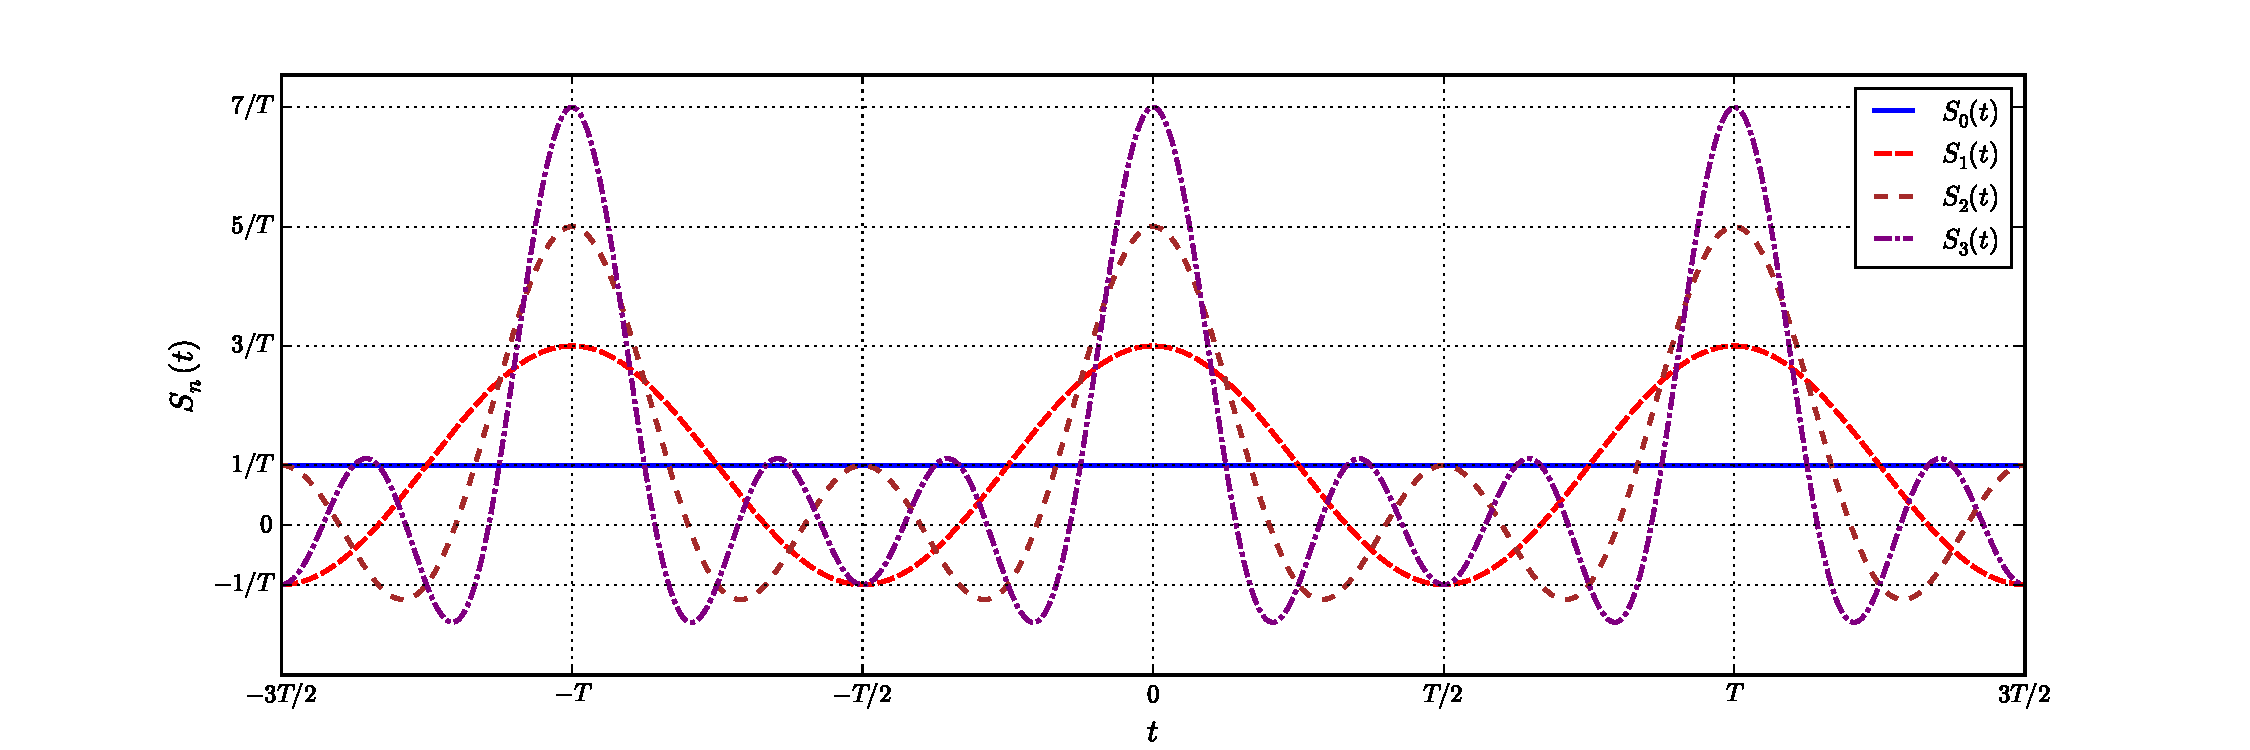
\includegraphics[scale=0.4]{figs/fig-Fourier-serie-Dirac}
\caption{Serie de Fourier de la Delta de Dirac con per'iodo $T=2\pi$, truncada hasta $n=4$.}
\label{im:delta}
\end{figure}


\chapter{La transformada de Fourier}

Las series de Fourier permiten representar una funci'on \textit{peri'odica} como superposici'on de funciones seno y coseno (o exponenciales de argumento imaginario). Es posible extender el m'etodo de expansi'on de Fourier al caso de funciones no-peri'odicas, resultando las llamadas \textbf{integrales de Fourier}. Podemos entender estas integrales de Fourier como el \textit{l'imite cont'inuo} de las series de Fourier.

Consideremos una funci'on $f(t)$ de periodo $T$, y como intervalo fundamental a $(-T/2,T/2)$. Entonces, usando (\ref{ftpT}) y (\ref{fnpT}) podemos escribir
\begin{equation}\label{fcont1}
f(t) =\sum_{n = -\infty}^\infty\left[\frac{1}{T}\int_{-T/2}^{T/2} f(\xi) e^{-i\omega_n\xi}\, d\xi\right] e^{i\omega_nt}.
\end{equation}
Equivalentemente, podemos expresar la suma en (\ref{fcont1}) en t'erminos de la frecuencias $\omega_n$ y la diferencia (en este caso, constante) entre ellas $\Delta\omega:=\omega_{n+1}-\omega_n=2\pi/T$:
\begin{equation}
f(t) =\sum_{\omega_n = -\infty}^\infty\left[\frac{1}{2\pi}
\int_{-T/2}^{T/2} f(\xi) e^{-i\omega_n\xi}\,d\xi\right] e^{i\omega_n t}\Delta\omega.
\end{equation}
En el l'imite $T\to\infty$, (y por lo tanto $\Delta\omega\to 0$), la funci'on $f(t)$ puede considerarse como una funci'on no-peri'odica arbitraria definida en todo el intervalo $(-\infty,\infty)$. Por otro lado, la suma se transforma en una integral\footnote{Recuerde la definici'on de integral de Riemann: $\int_a^bf(x)\,dx:=\lim_{\Delta x_i\to 0}\sum_{x_i}f(x_i)\Delta x_i$.}. Por lo tanto, en este l'imite obtenemos la identidad
\begin{equation}\label{idfnp}
f(t) =\int_{-\infty}^\infty\left[\frac{1}{2\pi}\int_{-\infty}^\infty
 f(\xi) e^{-i\omega\xi}\,d\xi\right] e^{i\omega t}\,d\omega,
\end{equation}
a partir de la cual podemos definir la \textbf{transformada de Fourier} de la funci'on $f(t)$ como
\begin{equation}\label{TFf}
\boxed{\tilde{f}(\omega) :=\int_{-\infty}^\infty f(t) e^{-i\omega t}\,dt,}
\end{equation}
de modo que la ``transformada inversa'' resulta ser
\begin{equation}\label{TFIf}
\boxed{f(t)=\frac{1}{2\pi}\int_{-\infty}^\infty\tilde{f}(\omega) e^{i\omega t} \,d\omega.}
\end{equation}



Observaciones:

\begin{itemize}
\item Cuidado! La derivaci'on anterior es ``heur'istica'' (e.d. no rigurosa). 
\item Otras notaciones: $\tilde{f}(\omega)=g(\omega)={\cal F}(f)(\omega)$.
\item El factor $1/2\pi$ en la definici'on (\ref{TFIf}) es hasta cierto punto convencional. Lo importante es la identidad (\ref{idfnp}). Por ejemplo, en lugar de estos factores, podr'ia introducirse $\alpha$ en (\ref{TFf}) y $1/2\pi\alpha$ en (\ref{TFIf}), con una constante $\alpha$ arbitraria. Otras elecciones populares son $\alpha=1$ y $\alpha=1/\sqrt{2\pi}$.
\item Note que en (\ref{TFIf}) la integral se extiende sobre ``frecuencias positivas y negativas''.
\item Compare (\ref{TFf}) con la definici'on de la \textbf{transformada de Laplace}: $F(s):=\int_0^\infty f(t)e^{-st}dt$.
\item En F'isica es costumbre denotar, en el caso en que se considere una funci'on de la posici'on, $f(t)\to f(x)$ y usar el \textit{n'umero de onda} $k$ en lugar de la frecuecia $\omega$, de modo que la expansi'on adopta la forma $f(x)=(1/{2\pi})\int_{-\infty}^\infty\tilde{f}(k) e^{ikx} \,dk.$
\end{itemize}

\subsection{Ejemplo: Distribuci'on Gaussiana}
Considere la \textbf{distribuci'on gaussiana} definida por
\begin{equation}\label{fgauss}
f(t):=N e^{-\alpha t^2}, \qquad \alpha>0,
\end{equation}
entonces su transformada de Fourier es dada por
\begin{align}
\tilde{f}(\omega)=&N\int_{-\infty}^{\infty}e^{-\alpha t^2} e^{-i \omega t}dt\notag \\
=&N\int_{-\infty}^{\infty}e^{-\alpha t^2-i\omega t} dt.
\end{align}
Notando que
\begin{align}
-\alpha t^2-i\omega t=&-\alpha \left(t^2+\frac{\omega}{\alpha}t\right) \notag \\
=&-\alpha\left(t^2+\frac{\omega}{\alpha}t+\left(\frac{i\omega}{2\alpha}\right)^2-\left(\frac{i\omega}{2\alpha}\right)^2\right) \notag \\
=&-\alpha \left( t+\frac{i\omega}{2\alpha} \right)^2+\alpha\left(\frac{i\omega}{2\alpha}\right)^2\notag \\
=&-\alpha \left( t+\frac{i\omega}{2\alpha} \right)^2-\left(\frac{\omega^2}{4\alpha}\right),
\end{align}
se halla entonces que
\begin{align}
\tilde{f}(\omega)=&N\int_{-\infty}^{\infty}e^{-\alpha \left( t+\frac{i\omega}{2\alpha} \right)^2-\left(\frac{\omega^2}{4\alpha}\right)}dt\notag\\
=&N e^{-\frac{\omega^2}{4\alpha}}\int_{-\infty}^{\infty}e^{-\alpha \left( t+\frac{i\omega}{2\alpha} \right)^2}dt,
\end{align}
pero haciendo el cambio de variables $x:=\sqrt{\alpha}(t+i\omega/4\alpha)$, entonces $dx=\sqrt{\alpha}\,dt$, luego
\begin{align}
\tilde{f}(\omega)=N e^{-\frac{\omega^2}{4\alpha}}\int_{-\infty}^{\infty}e^{-x^2} \frac{dx}{\sqrt{\alpha}}.
\end{align}
Adem'as, recordando que
\begin{align}
\int_{-\infty}^{\infty}e^{-x^2}dx=\sqrt{\pi},
\end{align}
encontramos que
\begin{equation}\label{Tfgauss}
\tilde{f}(\omega)=N\sqrt{\frac{\pi}{\alpha}}e^{-\frac{\omega^2}{4\alpha}}.
\end{equation}
\begin{figure}[h]
\centering
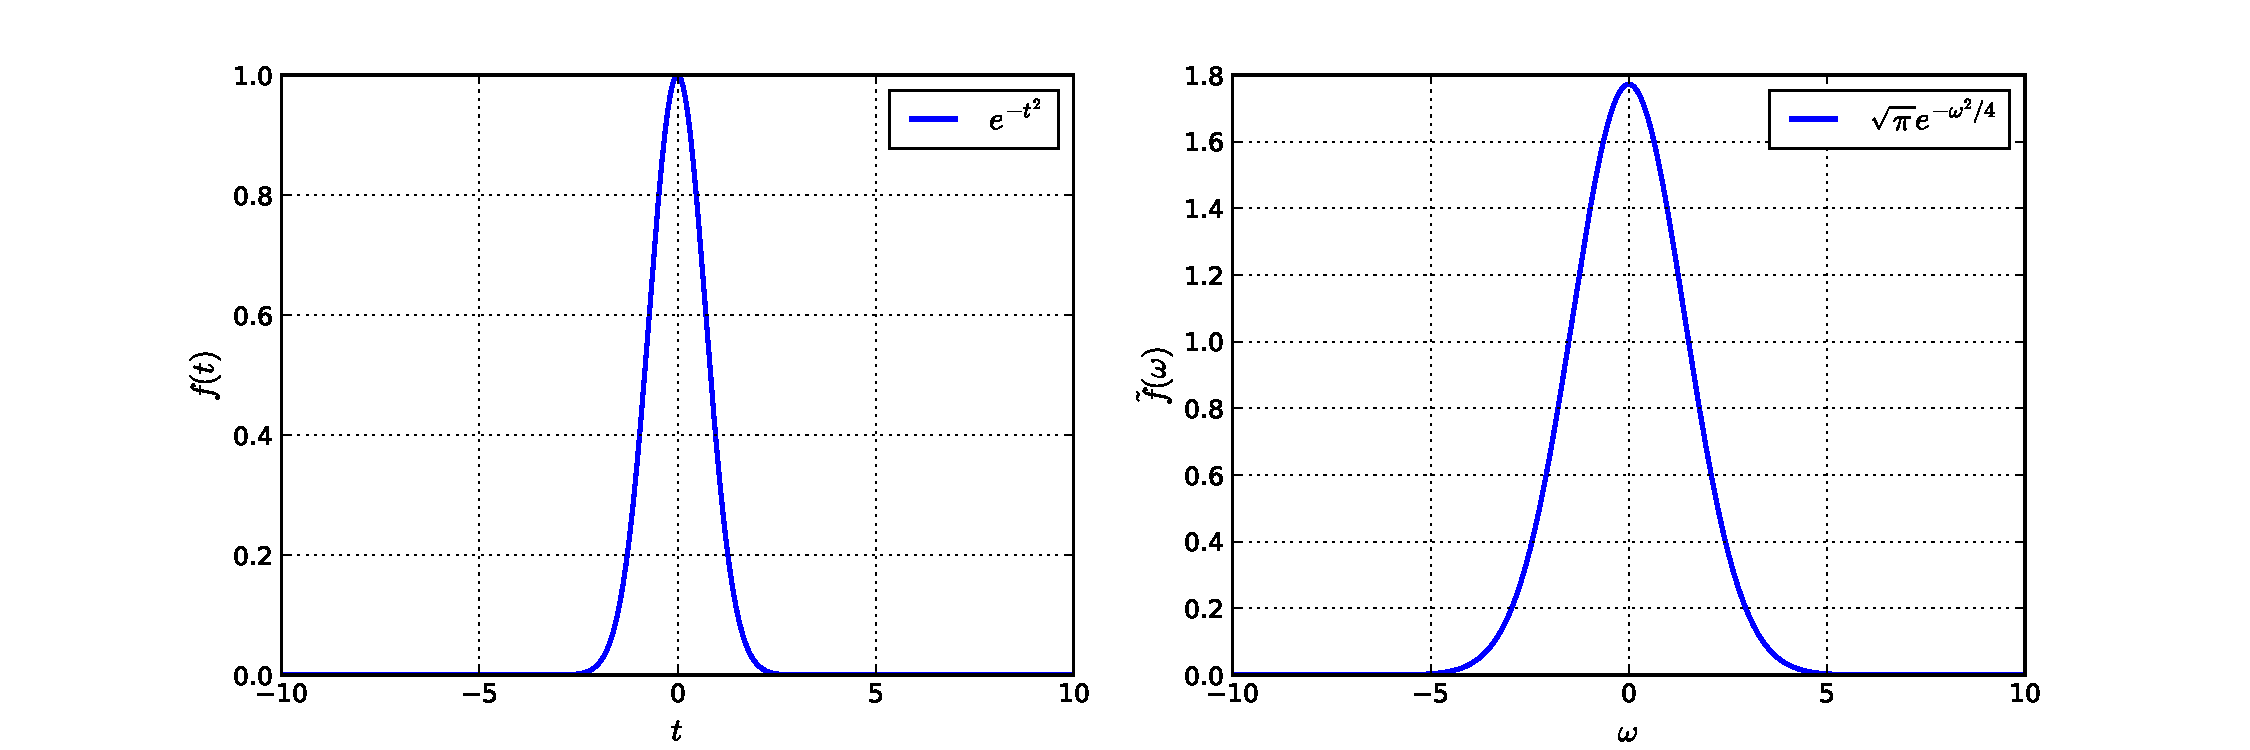
\includegraphics[scale=0.4]{figs/fig-Fourier-Gaussiana.pdf}
\caption{Distribuci'on gaussiana y su transformada de Fourier con $N=1$ y $\alpha=1$.}
\label{im:gaussiana}
\end{figure}


\section{Propiedades de la Transformada de Fourier} 
\subsection{Delta de Dirac}
\begin{align}
{\cal F}[\delta(t-\xi)] 
 &=\int_{-\infty}^\infty\delta(t-\xi) e^{-i\omega t}\,dt 
\\
 &=e^{-i\omega\xi} \label{Fd}
\end{align}
\begin{equation}
\boxed{ 
\delta(t-\xi) =\frac{1}{2\pi}\int_{-\infty}^\infty e^{i\omega (t-\xi)}\,d\omega. 
 }
\end{equation}
%
\subsection{Transformada de Fourier de la derivada de una funci'on}
\begin{align}
{\cal F}[f'(t)]
 &=\int_{-\infty}^\infty f'(t) e^{-i\omega t}\,dt \\
 &=\left[ f(t) e^{-i\omega x}\right]_{-\infty}^\infty
 -\int_{-\infty}^\infty (-i\omega) f(t) e^{-i\omega t}\,dt \\
 &=\left[ f(t) e^{-i\omega x}\right]_{-\infty}^\infty+ i\omega\int_{-\infty}^\infty f(t) e^{-i\omega t}\,dt \\
 &= i\omega{\cal F}[f(t)]+\left. f(t) e^{-i\omega x}\right|_{-\infty}^\infty.\label{eq:trans-fourier-derivada-gen}
\end{align}
Entonces, \textit{si la funci'on $f(t)$ se anula en el infinito}, es decir si $\lim_{t\to\pm\infty}f(t)=0$, tendremos que
\begin{equation}
\boxed{ 
{\cal F}\left[f'(t)\right] = (i\omega){\cal F}[f(t)]. \label{eq:trans-fourier-derivada-esp}
 } 
\end{equation} 
Aplicaci'on sucesiva de esta relaci'on, bajo las mismas condiciones, conduce a
\begin{equation}
\boxed{ 
{\cal F}\left[f^{(n)}(t)\right] = (i\omega)^n{\cal F}[f(t)]. 
 } 
\end{equation} 



\subsubsection{Ejemplo: Funci'on escal'on.}
Sea la funci'on escal'on $H(t)$ tal que
\begin{equation}
H_c(t) := 
\begin{cases}
0, &\text{si }t < c,\\
1, &\text{si }t > c
\end{cases},
\end{equation}

\begin{figure}[h]
\centering
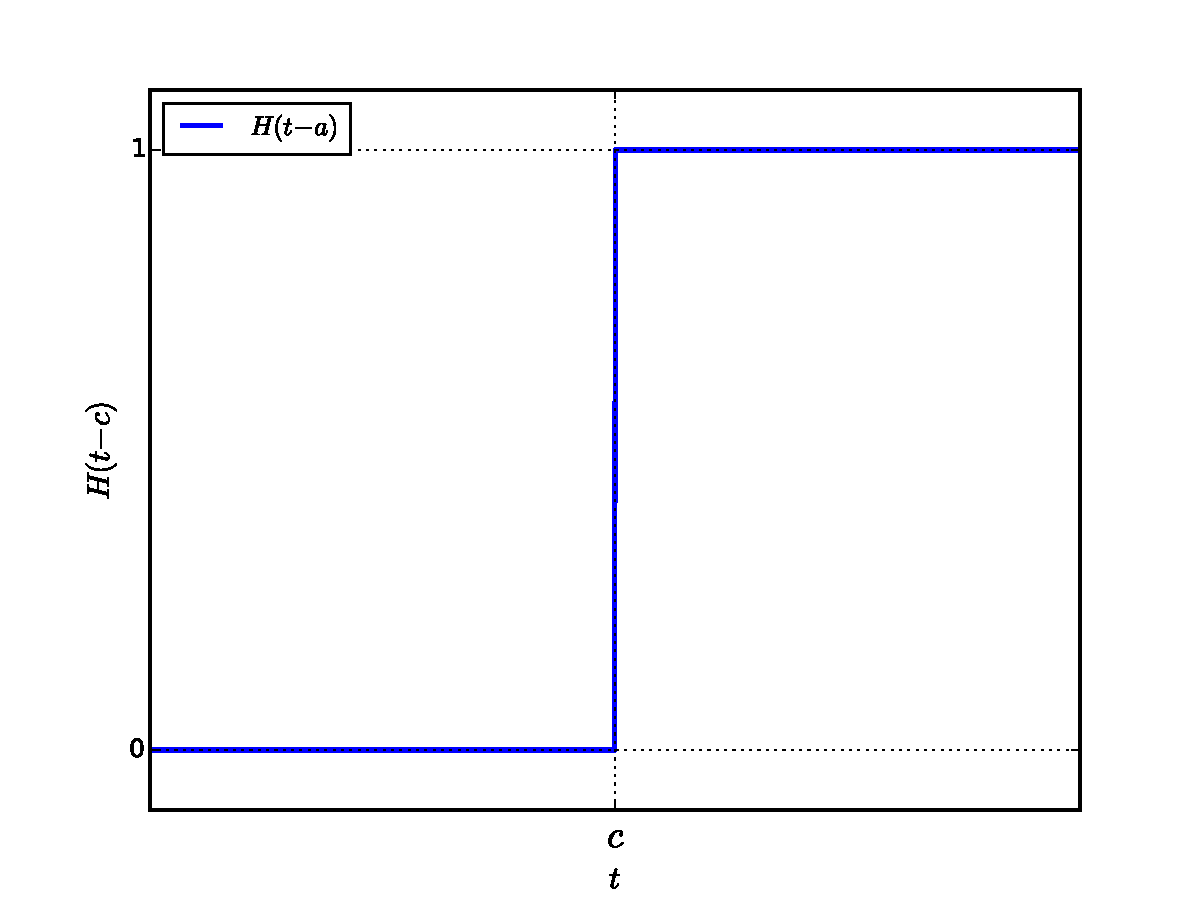
\includegraphics[scale=0.4]{figs/fig-funcion-escalon.pdf}
\caption{Funci'on escal'on.}
\label{im:escalon}
\end{figure}
con la interesante propiedad que
\begin{equation}
\frac{dH}{dt}(t) = \delta(t-c).
\end{equation}
Es de relevancia mencionar que ingenuamente podr'iamos pasar por alto el hecho que la funci'on escal'on no satisface la hip'otesis que $\lim_{t\to\pm\infty}H(t-c)=0$ y recordando \eqref{Fd} podr'iamos pretender calcular la transformada de Fourier simplemente usando la expresi'on \eqref{eq:trans-fourier-derivada-esp}, lo que nos conducir'ia err'oneamente a que
\begin{equation}
\boxed{ {\cal F}[H(t-c)] =\frac{1}{i\omega} e^{-i c\omega}.}
\end{equation}
Sin embargo, al emplear directamente la definici'on de la transformada de Fourier vemos que
\begin{align}
{\cal F}[H](\omega)=&\int_{-\infty}^{\infty}H(t)e^{-i\omega t}dt\notag \\
=&\int_{c}^{\infty}1\cdot e^{-i\omega t}dt\notag \\
=&\left.\frac{e^{-i\omega t}}{-i\omega}\right|_{c}^{\infty}, \label{TFH}
\end{align}
y debido a que
\begin{align}
\left.\frac{e^{-i\omega t}}{-i\omega}\right|_{\infty}=\lim_{t \rightarrow \infty}\frac{e^{-i\omega t}}{-i\omega}
\end{align}
no existe (el l'imite no tiende a un valor 'unico), entonces se concluye que la transformada de Fourier de la funci'on escal'on tampoco. Sin embargo, la relaci'on  completa \eqref{eq:trans-fourier-derivada-gen} sigue siendo v'alida y suministra una expresi'on equivalente a \eqref{TFH}.
%
\subsection{Teorema de Convoluci'on}
El teorema de convoluci'on suministra una 'util relaci'on entre la transformada de Fourier de un producto de funciones y las transformadas de Fourier de cada una de las funcioes.
\begin{align}
{\cal F}[f_1(t)f_2(t)]
 &=\int_{-\infty}^\infty f_1(t)f_2(t) e^{-i\omega t}\,dt \\
 &=\frac{1}{2\pi}\int_{-\infty}^\infty f_1(t) \left(\int_{-\infty}^\infty\tilde{f}_2(\omega')
 e^{i\omega' t}\,d\omega'\right)e^{-i\omega t}\,dt \\
 &=\frac{1}{2\pi}\int_{-\infty}^\infty\left(\int_{-\infty}^\infty f_1(t) 
 e^{-i(\omega-\omega')t}\,dt\right)\tilde{f}_2(\omega')\,d\omega' \\
 &=\frac{1}{2\pi} \int_{-\infty}^\infty\tilde{f}_1(\omega-\omega')\tilde{f}_2(\omega)\,d\omega'.
\end{align}
Por lo tanto, 
\begin{equation}
\boxed{ \tilde{f}_{1\cdot 2}(\omega)=\frac{1}{2\pi} \int_{-\infty}^\infty\tilde{f}_1(\omega-\omega')\tilde{f}_2(\omega)\,d\omega' .
 } 
\end{equation}   
An'alogamente, la relaci'on entre las transformadas inversas es
\begin{equation}
{\cal F}^{-1}[\tilde{f}_1(\omega)\tilde{f}_2(\omega)]
=\int_{-\infty}^\infty f_1(\xi)f_2(t-\xi)\,d\xi .	
\end{equation}



\subsubsection{Ejemplo} Usando el teorema de convoluci'on podemos encontrar la transformada de Fourier de 
\begin{equation}
 f(t) =\frac{1}{t^4 + 5 t^2 + 4}. 
\end{equation}
\begin{equation}
 f(t) =\frac{1}{(t^2+1)(t^2+4)}
\end{equation}
\begin{equation}
{\cal F}\left[\frac{c}{t^2+c^2}\right] = \pi e^{-c |\omega|},\qquad\text{ para }c > 0. 
\end{equation}
\begin{align}
{\cal F}[f(t)]
 &={\cal F}\left[\frac{1}{t^2+1}\frac{1}{t^2+4}\right] 
\\
 &=\frac{1}{2\pi}\frac{\pi}{1}\frac{\pi}{2}\left(\int_{-\infty}^\infty e^{-|\eta|} e^{-2|\omega -\eta|}\,d\eta\right) 
\\
 &=\frac{\pi}{4}\left(\int_{-\infty}^0 e^\eta e^{-2|\omega -\eta|}\,d\eta
 +\int_0^\infty e^{-\eta} e^{-2|\omega -\eta|}\,d\eta\right)
\end{align}
Si $\omega > 0$,
\begin{align}
{\cal F}[f(t)]
 &=\frac{\pi}{4}\left(\int_{-\infty}^0 e^{-2\omega + 3\eta}\,d\eta
 +\int_0^\omega e^{-2\omega +\eta}\,d\eta
 +\int_\omega^\infty e^{2\omega - 3\eta}\,d\eta\right) 
\\
 &=\frac{\pi}{4}\left(\frac{1}{3} e^{-2\omega} + e^{-\omega}
 - e^{-2\omega} +\frac{1}{3} e^{-\omega}\right) 
\\
 &=\frac{\pi}{2}\left[ \frac{2}{3}e^{-\omega} -\frac{1}{3} e^{-2\omega}\right].
\end{align}
Si $\omega < 0$,
\begin{align}
{\cal F}[f(t)]
 &=\frac{\pi}{4}\left(\int_{-\infty}^\omega e^{-2\omega+3\eta}\,d\eta
 +\int_\omega^0 e^{2\omega -\eta}\,d\eta
 +\int_0^\infty e^{2\omega-3\eta}\,d\eta\right) 
\\
 &=\frac{\pi}{4}\left(\frac{1}{3} e^\omega - e^{2\omega}
 + e^\omega +\frac{1}{3} e^{2\omega}\right)\\
 &=\frac{\pi}{2}\left[\frac{2}{3}e^\omega -\frac{1}{3} e^{2\omega} \right].
\end{align}
Podemos expresar los resultados para ambos signos de $\omega$ como:
\begin{equation}
\boxed{ 
{\cal F}[f(t)] =\frac{\pi}{2}\left[\frac{2}{3} e^{-|\omega|} -\frac{1}{3} e^{-2|\omega|} \right].
 } 
\end{equation} 
Otra forma de encontrar la transformada de
\begin{equation}
f(t) =\frac{1}{t^4 + 5 t^2 + 4}
\end{equation}
es expandir la funci'on en fracciones parciales:
\begin{equation}
f(t) =\frac{1}{3}\frac{1}{t^2 + 1} -\frac{1}{3}\frac{1}{t^2 + 4},
\end{equation}
\begin{align}
{\cal F}[f(t)]
&=\frac{1}{3}{\cal F}\left[\frac{1}{t^2 + 1}\right]
-\frac{1}{3}{\cal F}\left[\frac{1}{t^2+4}\right]\\
&=\frac{1}{3}\frac{\pi}{1} e^{-|\omega|} -\frac{1}{3}\frac{\pi}{2} e^{-2|\omega|}.
\end{align}        

\subsection{Teorema de Parseval}
\begin{equation}
\boxed{
\int_{-\infty}^\infty |f(t)|^2\,dt=\frac{1}{2\pi}\int_{-\infty}^\infty |\tilde{f}(\omega)|^2\,d\omega.
 }
\end{equation}
    
\subsection{Ancho de la funci'on y su transformada}

Definimos el \textbf{valor medio} de $t$ respecto a la funci'on (distribuci'on) $f(t)$ como
\begin{equation}
\langle t \rangle:=\frac{\int f^{*}(t) t f(t)\,dt}{\int |f(t)|^{2}\, dt}=\frac{\int t |f(t)|^2\,dt}{\int |f(t)|^2\,dt}
\end{equation}
y, an'alogamente, el valor medio de $\omega$ respecto a la transformada $\tilde{f}(\omega)$ por
\begin{equation}
\langle \omega \rangle:=\frac{\int \tilde{f}^{*}(\omega) \omega \tilde{f}(\omega) d\omega}{\int |\tilde{f}(\omega)|^{2} d\omega}=\frac{\int \omega |\tilde{f}(\omega)|^2 d\omega}{\int |\tilde{f}(\omega)|^2 d\omega}.
\end{equation}
De forma similar, la \textbf{varianza} de $t$ respecto a $f(t)$ es definida por
\begin{equation}
(\Delta t)^2:=\frac{\int f^{*}(t)(t-\langle t \rangle)^2 f(t)\,dt}{\int |f(t)|^2\, dt}=\frac{\int (t- \langle t \rangle)^2 |f(t)|^2 t}{\int |f(t)|^2 dt}.
\end{equation}
Finalmente, la varianza de $\omega$ respecto a $\tilde{f}(\omega)$ es dada por:
\begin{equation}
(\Delta \omega)^2:=\frac{\int \tilde{f}^{*}(\omega)(\omega-\langle \omega \rangle)^2 \tilde{f}( \omega) d\omega}{\int |\tilde{f}(\omega)|^2 d\omega}=\frac{\int (\omega- \langle \omega \rangle)^2 |\tilde{f}(\omega)|^2 \omega}{\int |\tilde{f}(\omega)|^2 d\omega}.
\end{equation}


Sea $f(t)$ una funci'on tal que $\lim_{t \rightarrow \pm \infty} f(t)=0$ y $f'=df/dt$, entonces $\tilde{f'}=i \omega \tilde{f}$, y podemos escribir $\omega \tilde{f}=-i \tilde{f'}$. Por lo tanto
\begin{align}
(\Delta \omega)^2 \int |\tilde{f}|^2 d\omega =&\int |i\tilde{f'}+\langle \omega \rangle \tilde{f}|^2 d \omega \notag \\
=&\int |{\cal F}[if'+\langle \omega \rangle f]|^2 d\omega.
\end{align}
Pero empleando el teorema de Parseval se encuentra que
\begin{align}
(\Delta \omega)^2 \int |\tilde{f}|^2 d\omega &= 2\pi\int |if'+\langle \omega \rangle f]|^2 dt.
\end{align}
Recordando la desigualdad (triangular) de Schwarz, que establece que $\forall f_{1},f_{2}$ se cumple que
\begin{align}
\left( \int |f_{1}|^2 dt \right)\left( \int |f_{2}|^2 dt\right) \geq \left|\int f_{1}^{*}f_{2}dt\right|,
\end{align}
y considerando $f_{1}(t):=(t-\langle t \rangle)f(t)$ y $f_{2}(t):=if'(t)+\langle \omega \rangle f(t)$, se tiene que
\begin{align}
\left(\int |f|^2 dt \right) (\Delta t)^2 \cdot (\Delta \omega)^2 \left(\int |f|^2 dt \right)\geq
\left|\int f^{*}(t)(t-\langle t \rangle)\left(if'(t)+ \langle\omega\rangle f(t)\right) dt\right|^2.
\end{align}
Si definimos $I$ como la integral del segundo miembro de la ecuaci'on precedente, podemos hallar que
\begin{align}
I=&\int \left[ i f^{*}t f'+\langle \omega \rangle f^{*} t f-\langle t \rangle i f^{*}f'-\langle t \rangle \langle \omega \rangle |f|^2\right]dt  \notag \\
=&i\int \left(f^{*} t \frac{df}{dt}-\langle t \rangle f^{*} \frac{df}{dt} \right) dt+\langle \omega \rangle \langle t \rangle \int |f|^2 dt-\langle t \rangle \langle \omega \rangle \int |f|^2 dt\notag \\
=&i \int f^{*}(t-\langle t\rangle)\frac{df}{dt} dt.
\end{align}
Notando que
\begin{align}
{\rm Im}(I) &= \frac{1}{2}\int \left[ f^{*}(t-\langle t \rangle)\frac{df}{dt}+\left(\frac{df}{dt}\right)^{*}(t-\langle t \rangle)f\right]dt\notag \\
&= \frac{1}{2}\int \left( \frac{d}{dt}[f^{*}(t-\langle t \rangle)f]-f^{*}f\right)dt\notag \\
&= \left. \frac{1}{2} (t-\langle t \rangle)|f|^2 \right|_{-\infty}^{\infty}-\frac{1}{2}\int |f|^2 dt.
\end{align}
Para que $\int |f|^2 dt$ y $\langle t \rangle$ sean finitos, suponemos que $|f|^2\rightarrow 0$ y $t|f^2| \rightarrow 0$ cuando $t \rightarrow \pm \infty$. En tal caso
\begin{align}
{\rm Im}(I)=-\frac{1}{2}\int |f|^2 dt.
\end{align}
Adem'as, como $|I|^2=[{\rm Re}(I)]^2+[{\rm Im}(I)]^2\geq [{\rm Im}(I)]^2$, podemos escribir que
\begin{align}
(\Delta t)^2 (\Delta \omega)^2 \left(\int |f|^2 dt \right)^2 \geq [{\rm Im}(I)]^2= \frac{1}{4} \left( \int |f|^2 dt\right)^2,
\end{align}
de donde se deduce que
\begin{align}
(\Delta t)^2 \cdot (\Delta\omega)^2 \geq \frac{1}{4}
\end{align}
o, finalmente,
\begin{align}\label{DtDo}
\boxed{
\Delta t\cdot \Delta\omega\ge\frac{1}{2}.
}
\end{align}

\subsubsection{Ejemplo}
Un ejemplo instructivo es el caso de la funci'on gaussiana \eqref{fgauss}. En este caso un c'alculo simple muestra que
\begin{equation}
\langle t\rangle=0,  \qquad \Delta t =\frac{1}{2\sqrt{\alpha}}.
\end{equation}
Similarmente, para la transformada \eqref{Tfgauss}, que tiene la misma forma funcional, tendremos que
\begin{equation}
\langle\omega\rangle=0,  \qquad \Delta\omega =\sqrt{\alpha}.
\end{equation}
Verificamos que en ambos casos los valores medios son una medida del ``valor central'' y que la varianza cuantifica el ``ancho'' de cada distribuci'on. La distribuci'on gaussiana es especial en el sentido que \textit{satura la desigualdad} \eqref{DtDo}, ya que en este caso
\begin{equation}
\Delta t\cdot \Delta\omega =\frac{1}{2}.
\end{equation}
\section{Generalizaci'on a mayores dimensiones}
En $D$ dimensiones:
\begin{equation}
{\cal F}[f(\vec{x})]=\tilde{f}(\vec{k})
:= \int f(\vec{x})e^{i(\vec{k}\cdot\vec{x})}d^Dx,
\end{equation}
\begin{equation}
f(\vec{x}) = {\cal F}^{-1}(\tilde{f})
:= \frac{1}{(2\pi)^{D}}\int \tilde{f}(\vec{k})e^{-i(\vec{k}\cdot\vec{x})}d^Dk.
\end{equation}

*** cambio convenci'on! listo hasta aqu'i ***


\section{Transformada de Fourier seno y coseno}










